\documentclass[border=4pt,12pt]{standalone}
% House style for redrawn exam diagrams (diagram-v4: 0.4pt lines, filled -latex arrows, fine dashes; stipple and hatching drawn as real dots/lines (no PDF/SVG patterns, so they render in every browser and at any scale); transparent background). Every figure \input's this.
\usepackage{amsmath,amssymb}
\usepackage{txfonts}
\usepackage{pdfrender,xcolor}
% \halo{text}: label on shading. The shading stops just around each letter's outline (a thin knock-out that follows the
% glyphs, like the papers' typesetting), never a box. Owner: "I don't want a box around the text".
\newcommand{\halo}[1]{\leavevmode\rlap{\pdfrender{TextRenderingMode=2,LineWidth=2.2pt,LineJoinStyle=1,StrokeColor=white,FillColor=white}#1}#1}
\usepackage{tikz,pgfplots}
\pgfplotsset{compat=1.18}
\usetikzlibrary{arrows.meta,calc,angles,quotes,patterns,patterns.meta,intersections,positioning,decorations.markings,shapes.geometric}
% Stipple and hatching are drawn as actual dots / lines clipped to the region (path picture), NOT as pattern fills:
% SVG <pattern> fills vanish or blur when browsers scale the image, so the owner could not see the shading.
% Each dot is a 0.72pt square (keeps SVGs small; reads as a dot at print size). Dots sit on one global staggered grid, so neighbouring regions line up.
\makeatletter
\newdimen\ex@x \newdimen\ex@y \newdimen\ex@xa \newdimen\ex@ya \newdimen\ex@xb \newdimen\ex@yb \newcount\ex@row
\def\exam@stipplecolor{black!75}\def\exam@dotr{0.42pt}\def\exam@dotgap{2.5}
\def\ex@rowdots{\ifdim\ex@x<\ex@xb \pgfpathrectangle{\pgfqpoint{\dimexpr\ex@x-0.36pt\relax}{\dimexpr\ex@y-0.36pt\relax}}{\pgfqpoint{0.72pt}{0.72pt}}\advance\ex@x by \exam@dotgap pt\relax\expandafter\ex@rowdots\fi}
\def\exam@stipple{%
  \pgftransformreset% dots are sized in real points even inside scaled pictures
  \pgfpointanchor{path picture bounding box}{south west}\ex@xa=\pgf@x \ex@ya=\pgf@y
  \pgfpointanchor{path picture bounding box}{north east}\ex@xb=\pgf@x \ex@yb=\pgf@y
  \pgfsetfillcolor{\exam@stipplecolor}\pgfmathsetmacro\ex@h{\exam@dotgap/2}%
  \pgfmathtruncatemacro\ex@r{floor(\ex@ya/\ex@h)-1}\ex@row=\ex@r\relax
  \ex@y=\ex@r\dimexpr\ex@h pt\relax
  \loop\ifdim\ex@y<\ex@yb
    \pgfmathtruncatemacro\ex@c{floor(\ex@xa/\exam@dotgap)-1}\ex@x=\ex@c\dimexpr\exam@dotgap pt\relax
    \ifodd\ex@row \advance\ex@x by \ex@h pt\fi
    \ex@rowdots
    \advance\ex@y by \ex@h pt \advance\ex@row by 1
    \ifnum\numexpr\ex@row-(\ex@row/4)*4\relax=0 \pgfusepath{fill}\fi% flush every 4 rows: bounded TeX memory, few clip copies in the SVG
  \repeat\pgfusepath{fill}}
\newdimen\ex@d
\def\exam@hatch#1{% #1 = 1 for /, -1 for \ ; lines 45 degrees, 3pt apart
  \pgftransformreset
  \pgfpointanchor{path picture bounding box}{south west}\ex@xa=\pgf@x \ex@ya=\pgf@y
  \pgfpointanchor{path picture bounding box}{north east}\ex@xb=\pgf@x \ex@yb=\pgf@y
  \ex@d=\dimexpr\ex@yb-\ex@ya\relax \ex@x=\dimexpr\ex@xa-\ex@d\relax
  \loop\ifdim\ex@x<\ex@xb
    \ifnum#1>0 \pgfpathmoveto{\pgfqpoint{\ex@x}{\ex@ya}}\pgfpathlineto{\pgfqpoint{\dimexpr\ex@x+\ex@d\relax}{\ex@yb}}%
    \else \pgfpathmoveto{\pgfqpoint{\ex@x}{\ex@yb}}\pgfpathlineto{\pgfqpoint{\dimexpr\ex@x+\ex@d\relax}{\ex@ya}}\fi
    \advance\ex@x by 4.24pt
  \repeat
  \pgfsetlinewidth{0.4pt}\pgfsetstrokecolor{black}\pgfusepath{stroke}}
\def\examstipple{\exam@stipple}\def\examhatch{\exam@hatch}\def\examsetstipplecolor#1{\def\exam@stipplecolor{#1}}\def\examsetdotgap#1{\def\exam@dotgap{#1}}
\makeatother
% (legacy pattern kept for old files)
% staggered stipple like the NESA papers' dotted shading
\pgfdeclarepatternformonly{exam stipple}{\pgfpointorigin}{\pgfqpoint{2.2pt}{2.2pt}}{\pgfqpoint{2.2pt}{2.2pt}}{%
  \pgfpathcircle{\pgfqpoint{0.55pt}{0.55pt}}{0.42pt}\pgfpathcircle{\pgfqpoint{1.65pt}{1.65pt}}{0.42pt}\pgfusepath{fill}}
\tikzset{
  every picture/.style={line width=0.6pt, >={Latex[length=2mm,width=1.3mm]}},
  curve/.style={line width=0.6pt},
  open arrow/.style={-{Latex[length=2mm,width=1.3mm]}},  % owner: filled -latex heads everywhere, no open chevrons
  aux/.style={dash pattern=on 2pt off 1.5pt, line width=0.6pt},
  shade/.code={\def\exA{#1}\def\exB{none}\ifx\exA\exB\else\pgfkeysalso{fill=black!18}\fi},
  shade/.default=on,
  shade dots/.style={fill=none, path picture={\examstipple}},
  stipple color/.code={\examsetstipplecolor{#1}},
  stipple gap/.code={\examsetdotgap{#1}},
  shade dense dots/.style={fill=none, stipple gap=1.6, path picture={\examstipple}},
  shade hatch/.style={fill=none, path picture={\examhatch{1}}},
  shade hatch reverse/.style={fill=none, path picture={\examhatch{-1}}},
  shade solid/.style={fill=black},
  pt/.style={circle, fill, inner sep=1.1pt},
  open pt/.style={circle, draw, fill=white, inner sep=1.1pt},
}
\pgfplotsset{
  exam axes/.style={axis lines=middle, axis line style={->}, xlabel={$x$}, ylabel={$y$},
    xlabel style={anchor=west}, ylabel style={anchor=south}, tick label style={font=\small},
    every axis plot/.append style={line width=0.6pt, black}, samples=200, clip=false,
    enlargelimits=false, axis on top},
}

\begin{document}
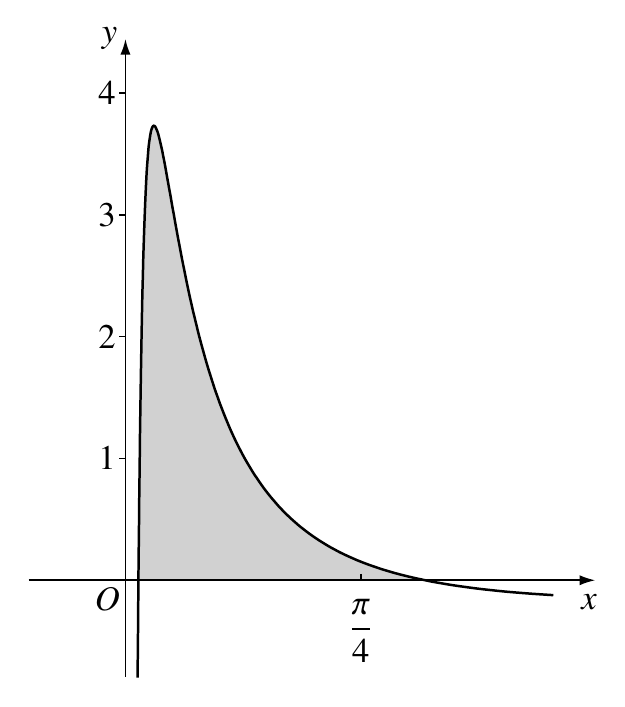
\begin{tikzpicture}[x=0.0127cm,y=-0.0127cm,font=\fontsize{12.5}{15.0}\selectfont]
\fill[shade] plot[smooth] coordinates {(135.0,582.5) (135.4,534.5) (135.9,489.8) (136.4,448.4) (136.9,410.2) (137.5,374.9) (138.0,342.6) (138.6,313.1) (139.2,286.2) (139.8,261.8) (140.4,239.9) (141.1,220.3) (141.8,203.0) (142.5,187.7) (143.2,174.4) (144.0,163.0) (144.8,153.3) (145.6,145.4) (146.5,139.1) (147.3,134.2) (148.2,130.8) (149.2,128.7) (150.2,127.8) (151.2,128.1) (152.2,129.4) (153.3,131.8) (154.4,135.1) (155.6,139.2) (156.8,144.1) (158.1,149.7) (159.4,156.0) (160.7,162.9) (162.1,170.3) (163.5,178.3) (165.0,186.6) (166.6,195.3) (168.2,204.4) (169.8,213.7) (171.5,223.4) (173.3,233.2) (175.2,243.2) (177.1,253.3) (179.1,263.5) (181.1,273.8) (183.2,284.1) (185.4,294.5) (187.7,304.8) (190.1,315.1) (192.5,325.4) (195.1,335.5) (197.7,345.6) (200.4,355.5) (203.2,365.3) (206.1,375.0) (209.2,384.5) (212.3,393.8) (215.5,403.0) (218.9,412.0) (222.4,420.7) (226.0,429.3) (229.7,437.6) (233.6,445.7) (237.6,453.6) (241.7,461.3) (246.0,468.7) (250.5,475.9) (255.1,482.9) (259.9,489.6) (264.9,496.1) (270.0,502.4) (275.3,508.4) (280.8,514.2) (286.5,519.8) (292.4,525.1) (298.6,530.2) (304.9,535.1) (311.5,539.8) (318.3,544.2) (325.3,548.5) (332.6,552.5) (340.2,556.3) (348.0,560.0) (356.2,563.4) (364.6,566.7) (373.3,569.7) (382.3,572.6) (391.7,575.3) (401.4,577.9) (411.4,580.3) (421.8,582.5)} -- cycle;
\draw[->] (25,582.5)--(592,582.5); \draw[->] (122,679)--(122,41);
\draw[line width=0.9pt] plot[smooth] coordinates {(134.1,680.0) (134.5,640.0) (134.8,601.9) (135.1,565.7) (135.5,531.3) (135.8,498.7) (136.2,467.9) (136.5,438.7) (136.9,411.2) (137.3,385.3) (137.7,360.9) (138.1,338.0) (138.5,316.6) (138.9,296.6) (139.4,277.9) (139.8,260.6) (140.3,244.5) (140.8,229.7) (141.3,216.1) (141.8,203.6) (142.3,192.3) (142.8,182.0) (143.3,172.7) (143.9,164.4) (144.5,157.1) (145.0,150.7) (145.6,145.1) (146.3,140.4) (146.9,136.5) (147.5,133.4) (148.2,131.0) (148.9,129.2) (149.6,128.2) (150.3,127.8) (151.0,128.0) (151.8,128.7) (152.5,130.1) (153.3,131.9) (154.2,134.2) (155.0,136.9) (155.8,140.1) (156.7,143.8) (157.6,147.7) (158.6,152.1) (159.5,156.8) (160.5,161.7) (161.5,167.0) (162.5,172.6) (163.5,178.4) (164.6,184.4) (165.7,190.6) (166.9,197.0) (168.0,203.6) (169.2,210.4) (170.5,217.3) (171.7,224.3) (173.0,231.4) (174.3,238.6) (175.7,245.9) (177.1,253.3) (178.5,260.7) (180.0,268.2) (181.5,275.6) (183.0,283.1) (184.6,290.7) (186.2,298.2) (187.9,305.7) (189.6,313.2) (191.4,320.6) (193.2,328.0) (195.0,335.4) (196.9,342.7) (198.9,350.0) (200.9,357.2) (202.9,364.3) (205.0,371.3) (207.2,378.3) (209.4,385.2) (211.6,392.0) (214.0,398.7) (216.3,405.2) (218.8,411.7) (221.3,418.1) (223.9,424.4) (226.5,430.6) (229.2,436.6) (232.0,442.6) (234.9,448.4) (237.8,454.1) (240.8,459.7) (243.9,465.1) (247.1,470.4) (250.3,475.7) (253.7,480.7) (257.1,485.7) (260.6,490.6) (264.2,495.3) (267.9,499.9) (271.7,504.3) (275.5,508.7) (279.5,512.9) (283.6,517.0) (287.8,521.0) (292.1,524.8) (296.5,528.6) (301.1,532.2) (305.7,535.7) (310.5,539.1) (315.4,542.4) (320.4,545.5) (325.5,548.6) (330.8,551.5) (336.2,554.4) (341.8,557.1) (347.5,559.7) (353.4,562.3) (359.4,564.7) (365.5,567.0) (371.9,569.2) (378.3,571.4) (385.0,573.4) (391.8,575.4) (398.8,577.2) (406.0,579.0) (413.4,580.7) (421.0,582.3) (428.7,583.9) (436.7,585.3) (444.9,586.7) (453.2,588.0) (461.8,589.2) (470.7,590.4) (479.7,591.5) (489.0,592.5) (498.5,593.5) (508.3,594.4) (518.3,595.2) (528.6,596.0) (539.2,596.7) (550.0,597.4)};
\draw (116,460.6)--(122,460.6); \node[anchor=east,inner sep=0] at (113,460.6) {$1$};
\draw (116,338.7)--(122,338.7); \node[anchor=east,inner sep=0] at (113,338.7) {$2$};
\draw (116,216.8)--(122,216.8); \node[anchor=east,inner sep=0] at (113,216.8) {$3$};
\draw (116,94.9)--(122,94.9); \node[anchor=east,inner sep=0] at (113,94.9) {$4$};
\draw (357.5,576)--(357.5,582.5); \node[anchor=north,inner sep=0] at (357.5,601) {$\dfrac{\pi}{4}$};
\node[anchor=base,inner sep=0] at (104,613) {$O$}; \node[anchor=base,inner sep=0] at (585,612) {$x$}; \node[anchor=base,inner sep=0] at (106,45) {$y$};\end{tikzpicture}
\end{document}
